\chapter{腹 水}

腹水是指腹腔内游离液体积存过多。引起腹水的病因很多(表\ref{tab28-1})。据国内多组统计,最常见的腹水病因依次为肝硬化、恶性肿瘤、结核性腹膜炎,三种病因合共占全部腹水病例90\%~95\%。

\begin{table}[htbp]
\centering
\caption{腹水疾病的分类}
\label{tab28-1}

\includegraphics[width=5.95833in,height=4.33333in]{./images/Image00152.jpg}
\end{table}

\section{【确定腹水的存在】}

少量腹水(1000ml以下)可无症状;中等量以上腹水,常有腹胀;大量腹水时可出现呼吸困难。

确定腹水存在首先依靠体格检查。检查腹水可取仰卧位、侧卧位及肘膝位三种不同体位。大量腹水时,仰卧位见腹部两侧膨胀形如蛙腹,叩诊有波动感。中度腹水采用左右侧卧位相交替叩诊,可检出移动性浊音。少量腹水应取肘膝位进行叩诊,若平卧时脐部叩诊鼓音,而肘膝位变为浊音,提示有腹水存在。当腹水量少时,物理诊断常不易检出。如腹腔有粘连,腹水可被包裹分隔,影响流动,此时移动性浊音不明显。

B超检查是诊断腹水敏感而简便的方法,并可鉴别腹水是游离还是分隔,其他含液体的结构如卵巢囊肿、腹腔囊肿、脓肿或血肿亦可通过B超被发现和鉴别。

腹水穿刺是确定腹水存在最直接的方法,并可观察腹水外观及作腹水化验。

腹水与腹胀的鉴别 腹水必须与其他原因所致的腹部膨胀相鉴别:

\subsection{(一)巨大卵巢囊肿}

可引起高度腹部膨胀,叩诊浊音与波动感,易与腹水相混淆。巨大卵巢囊肿有以下特征:①患者仰卧时,肠被压向腹后部与两侧,因此前腹叩诊呈浊音、腹侧部呈鼓音;②腹部前后膨胀度大于两侧膨胀度;③脐下腹围大于脐部或脐上的腹围;④脐孔有上移现象;⑤脐至髂前上棘的距离两侧不相等;⑥囊肿的轮廓可明显触知,阴道检查提示囊肿起源于卵巢;⑦B超检查有助鉴别。

\subsection{(二)其他巨大腹腔囊肿与巨大肾积水}

大网膜、腹膜后或胰腺囊肿与肾积水,可达到极大的程度,而与腹水混淆。这些病变的特点是:①病史长,起病缓慢,无明显全身症状;②腹部膨大,但两侧不对称;③腰腹部(一侧或两侧)叩诊呈鼓音,该处并可听到肠鸣音;④X线钡餐透视发现胃肠受压现象,结合静脉肾盂造影等检查,可证明囊肿起源于腹腔内或腹膜后器官;⑤超声检查也有助鉴别。

\subsection{(三)肥胖}

肥胖的人除腹壁由于脂肪堆积增厚,致腹部呈球形膨胀外,身体其他各部位也有脂肪堆积现象。无蛙腹,脐下陷,也无移动性浊音。

\subsection{(四)肠胀气}

高度鼓肠时腹部膨胀,但叩诊呈鼓音,无移动性浊音。

\section{【腹水病因鉴别诊断的相关检查】}

\subsection{(一)病史和体格检查}

详细的病史询问及全面的体格检查多可提供引起腹水病因的线索,可根据提示优先选择有关的实验室及其他辅助检查。对疑有结核或肿瘤的妇女应常规作妇科检查,对疑有肿瘤者常规作直肠指检,男性必要时作前列腺检查。

伴随病征的鉴别诊断意义概述如下:

\subsubsection{1.腹水与水肿的关系}

\paragraph{(1)单纯腹水而无全身水肿,或腹水出现在其他部位水肿之前者:}

多见于肝硬化失代偿期,腹、盆腔脏器癌肿的腹膜转移,结核性腹膜炎,恶性淋巴瘤,肝或门静脉血栓形成等。

\paragraph{(2)腹水伴有全身水肿者:}

常发生于心、肾疾病,营养障碍等。

\paragraph{(3)腹水出现在下肢水肿之后者:}

应注意充血性心力衰竭、心包炎、营养障碍、下腔静脉阻塞的可能。

\subsubsection{2.腹水伴有黄疸}

轻度黄疸可见于门脉性肝硬化、充血性心力衰竭、肝静脉阻塞;深度黄疸可见于重症急性肝炎、坏死后性肝硬化、肝癌。

\subsubsection{3.腹水伴有肝大}

须考虑肝硬化、肝癌、充血性心力衰竭、心包炎、重症肝炎、下腔静脉或肝静脉阻塞等。

\subsubsection{4.腹水伴有脾大}

常见于肝硬化、门静脉阻塞。

\subsubsection{5.腹水伴有腹壁静脉曲张}

多见于肝硬化,门静脉、肝静脉、下腔静脉阻塞。侧胸壁静脉曲张显著,且下腹壁静脉血流方向自下而上者,有利于下腔静脉阻塞的诊断。下腹壁静脉血流方向向下者,则多为门静脉阻塞。

\subsubsection{6.腹水伴有腹部肿块}

应考虑结核性腹膜炎、腹腔恶性肿瘤,女性患者并须注意梅格斯(Meigs)综合征的可能。

\subsection{(二)需要常规进行的实验室及影像学检查}

\subsubsection{1.血、尿、粪常规检查}

外周血白细胞及血小板减少常见于肝硬化脾功能亢进,而白细胞增高、中性粒细胞增高提示自发性细菌性腹膜炎;大量尿蛋白见于肾病综合征;多次粪便潜血强阳性提示消化道肿瘤。

\subsubsection{2.肝功能检查、肝炎病毒血清标记物、AFP检查}

因为肝病是腹水的最常见病因,这些检查应列为常规。

\subsubsection{3.B超检查}

不仅可确定腹水的存在及量的多少,且可了解腹腔、腹膜后及盆腔脏器病变,亦可测定门静脉直径。

\subsection{(三)腹水的实验室检查}

是腹水病因鉴别诊断的重要步骤,即使有明显肝硬化的患者在初次住院时亦应常规检查,因为有10\%或更多住院的肝硬化患者有腹水合并感染,而腹水感染并不一定都有明显症状,而且肝硬化也可有引起腹水的其他并发症及共存病。

\subsubsection{1.常规检查}

根据腹水外观及常规化验(比重、蛋白质定性和定量、细胞计数和分类)可分为漏出液、渗出液、血性及乳糜性等。漏出液为淡黄清亮,比重低于1.018,Rivalta试验阴性,蛋白质定量少于25g/L,白细胞计数少于100×10\textsuperscript{6}
/L。渗出液常混浊或为脓黏性,比重高于1.018,Rivalta试验阳性,蛋白质定量大于30g/L,白细胞计数常在500×10\textsuperscript{6}
/L以上,白细胞分类有助渗出液病因鉴别。血性腹水外观暗红或淡红,镜下见大量红细胞,由穿刺引起的出血呈不均匀血性,有凝块可资鉴别。乳糜性腹水外观呈乳白混浊,首先要区别真性与假性乳糜腹水,真性乳糜腹水富含淋巴液,乳糜试验阳性;假性乳糜腹水常因坏死降解的肿瘤或炎症细胞碎片形成,放置后可分层、乳糜试验阴性。

血清-腹水白蛋白梯度(SAAG) 同时抽血及抽腹水分别作白蛋白含量测定,血清白蛋白浓度减去腹水白蛋白浓度之差即为SAAG。以往根据腹水总蛋白浓度、白细胞计数等指标将腹水分为漏出液和渗出液,但因腹水总蛋白浓度常受多种因素影响,如血清白蛋白浓度、利尿剂使用等,据统计约20\%无并发症的肝硬化患者和过半数使用大量利尿剂后的肝硬化患者的腹水总蛋白超过25g/L;相反,肝硬化腹水合并感染最常发生在腹水总蛋白低于10g/L者;心源性腹水患者腹水总蛋白常大于25g/L。近年国内外研究认为根据SAAG分为高SAAG(≥11g/L)和低SAAG(<11g/L)对腹水性质进行分类优于漏出液和渗出液的分类法,高SAAG常提示门脉高压引起的腹水,而低SAAG则不存在门脉高压(表\ref{tab28-2})\footnote{*肝硬化伴结核性腹膜炎或肝硬化伴腹膜转移癌}。以SAAG作为腹水分类指标时应注意由于腹水白蛋白浓度有时很低,故必须对实验室检测白蛋白的标准曲张下限作相应调整。我国目前尚未广泛推广使用SAAG作为腹水性质分类标准,有待积累经验。

腹水特殊外观的病因提示 ①血性腹水:最常见于癌性腹水,结核性腹膜炎腹水也可呈血性,但较少见。肝硬化偶见一过性血性腹水但少有持续。少数Budd-Chiari综合征有血性腹水。急性发病的血性腹水见于急性胰腺炎。当腹腔穿刺液为不凝固的血液时,称为血腹,最常见于肝癌破裂或异位妊娠破裂,亦有其他原因引起的肝、碑破裂等。②乳糜性腹水(见下文)。③胆汁性腹水(见下文)。

\begin{table}[htbp]
\centering
\caption{根据SAAG所作的腹水病因分类}
\label{tab28-2}
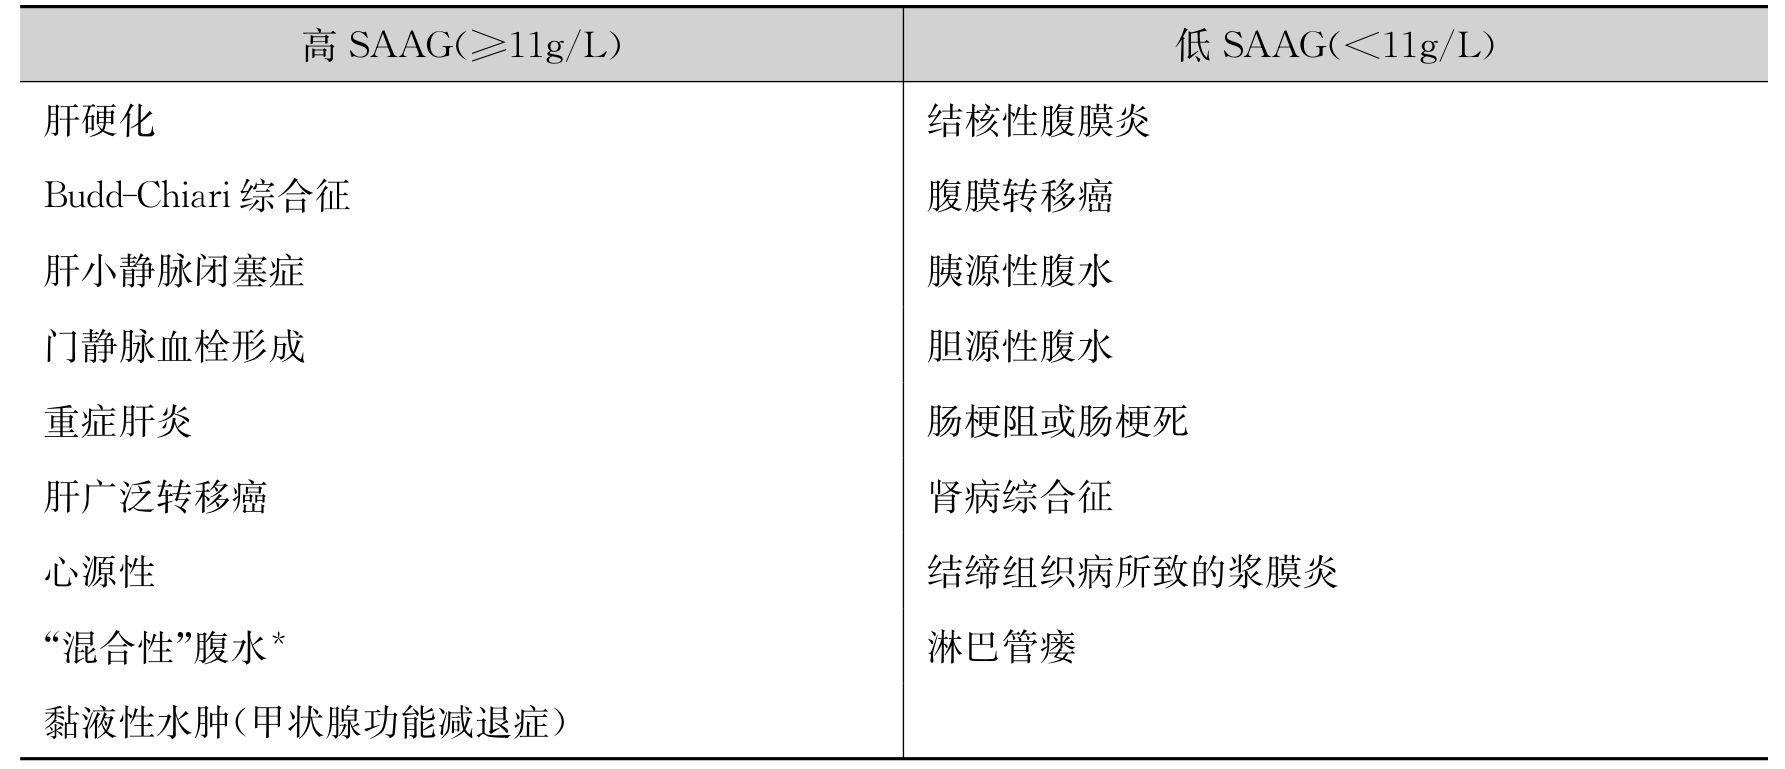
\includegraphics[width=5.9375in,height=2.55208in]{./images/Image00153.jpg}
\end{table}


\subsubsection{2.特殊检查}

\paragraph{(1)细菌培养:}

一般细菌培养,必要时加作厌氧菌培养,阳性对感染性腹水有确诊意义。强调必须采用床边血瓶接种培养法以提高阳性率。腹水找抗酸杆菌及结核菌培养阳性率很低,对结核性腹膜炎的临床诊断价值有限。

\paragraph{(2)细胞学检查:}

是诊断癌性腹水的重要依据。所取腹水量要够多(>250ml),待腹水细胞自然沉淀后离心,可提高阳性率。如高度怀疑而1次检查阴性者可重复抽取腹水检查。如方法得当,该检查对腹膜转移癌诊断的阳性率很高。

\paragraph{(3)葡萄糖含量:}

腹水葡萄糖含量低于空腹血糖值常提示腹水感染。

\paragraph{(4)乳酸脱氢酶(LDH):}

正常腹水与血清LDH比值为0.4左右,腹水感染或癌性腹水时,腹水LDH增高,腹水与血清LDH比值可>1.0。

\paragraph{(5)腺苷脱氨酶(ADA):}

结核性腹膜炎腹水ADA升高而其他疾病少有升高。

\paragraph{(6)肿瘤标记物:}

腹水癌胚抗原(CEA)及CA19-9在恶性肿瘤时常升高,有诊断参考价值。

\paragraph{(7)腹水淀粉酶:}

疑为胰性腹水,可查腹水淀粉酶,如腹水淀粉酶明显高于血淀粉酶含量,提示胰性腹水。

\subsection{(四)其他检查}

视诊断需要选择各种有关的实验室、影像学及其他辅助检查,目的是寻找引起腹水的原发病因。对于腹水病因诊断有困难的病例,腹腔镜检查结合直视下活检常可获确诊,特别是对结核性腹膜炎与腹膜转移癌的鉴别诊断、腹腔恶性肿瘤的诊断以及一些罕见疾病的发现,腹腔镜检查有其独特的价值。

\section{【腹水鉴别诊断的思路】}

以腹水为突出临床表现的鉴别诊断,一般根据腹水常规检查将腹水区分为漏出液和渗出液两大类,前者常见病因为肝硬化,其他病因有未有腹膜转移的肝癌、重症急性肝炎、心血管疾病、肾脏疾病、营养障碍疾病、甲状腺功能减退症等;后者常见于结核性腹膜炎和腹膜转移癌,其他病因有恶性淋巴瘤、胰源性腹水、胆源性腹水、结缔组织病或过敏性疾病引起的腹水Meigs综合征等。鉴别诊断先考虑引起腹水的常见病因,通过病史询问、体格检查,结合常规实验室和B超检查(见前述),一般可作出诊断或拟诊,必要时选择有关检查多可作出诊断。对常见病因不能解释的腹水病例,要考虑到少见病因并作有关检查,可避免延诊或误诊。

\protect\hypertarget{text00220.html}{}{}

\section{92 心血管疾病}

\subsection{一、慢性充血性右心衰竭}

慢性充血性右心衰竭发展至严重阶段时可发生腹水,但常伴有其他部位的重度水肿,病因多为风湿性。三尖瓣狭窄所引起的腹水常出现较早,且显著而持久,而其他部位的水肿较轻。此类患者多同时合并心源性肝硬化,表现为大量腹水,肝大、质硬,脾大等。腹水为漏出液性质,但腹水总蛋白含量多偏高,而SAAG≥11g/L。

\subsection{二、心包炎}

\subsubsection{(一)渗出性心包炎}

渗出性心包炎时可出现腹水,并伴有颈静脉怒张、肝大、肝颈反流征阳性、静脉压增高、下肢水肿等,酷似右心衰竭;但此病时心尖搏动消失、心音邈远,大量渗液时心浊音界向两侧增大、心浊音均呈绝对浊音,常有奇脉,与右心衰竭不同。

\subsubsection{(二)慢性缩窄性心包炎}

此病比较常见,患者多为青壮年人,病因最多为结核性,非特异性心包炎为其次,此外化脓性、放射治疗或心脏手术后等。主要症状为劳累后呼吸困难、腹水、下肢压陷性水肿、颈静脉怒张(吸气时更加扩张)、肝大、静脉压升高、脉压变小、奇脉、心脏搏动减弱、心音邈远等。患者临床上表现一种非常特殊的对照是:一方面并无心脏体积增大与心肌肥厚的体征,另一方面却有明显的淤血性肝大及其他体循环淤血现象。

慢性缩窄性心包炎常引起腹水,腹水的程度与全身水肿不相平衡,且常出现较早而较明显。部分患者可无全身水肿,而以腹水为主要表现,易误诊为肝硬化。其主要鉴别点是肝硬化无静脉压增高等体循环淤血的表现与奇脉,且失代偿期肝硬化有明显肝功能异常。X线检查发现心包钙化和心电图QRS波群、T波和P波改变有助慢性缩窄性心包炎诊断。CT或MRI可证实心包增厚,明确诊断。此病应注意与原发性限制型心肌病鉴别。

\subsection{三、原发性限制型心肌病}

本病临床表现与慢性缩窄性心包炎相似,可有肝大、腹水、足肿、心悸、气急等,但X线胸片上有心影增大(特别是呈球形增大)、心内膜有线状钙化而无心包钙化影、心电图呈心室肥厚、超声心动图见心尖部心脏闭塞及心内膜增厚等有助于与缩窄性心包炎相鉴别。对于诊断有困难病例可作心室造影和心内膜活栓(参见第52.3节)。

\subsection{四、Budd-Chiari综合征}

中文译文以往译为布-加综合征,后又改为柏-查综合征。该综合征是指肝静脉和(或)肝段下腔静脉狭窄或梗阻,致肝静脉和(或)下腔静脉血液回流障碍而表现为门静脉高压和(或)下腔静脉高压症候群。狭窄和梗阻主要由静脉隔膜和(或)血栓形成所致。大多数病因未明,少数可找到原发病因(如原发性血小板增多症、真性红细胞增多症、迁徙性血栓性静脉炎、口服避孕药、妊娠分娩后、系统性红斑狼疮、肾病综合征等易引起血液凝固异常的疾病,静脉癌性栓塞,肝脏病变、心包或纵隔病变侵犯或外压静脉等)。本病在我国并不少见,可见于任何年龄段,但多发于20~40岁,男女患病大致相等。其病程经过可分为急性和慢性两型。急性型少见(约占5\%),起病急骤,表现为急性腹痛、肝大和触痛、腹水及轻度黄疸,肝静脉完全闭塞时常出现肝衰竭,多死于肝性脑病。慢性型发展较慢,可先出现上腹痛、肝大和消化不良症状,亦可呈隐袭起病。临床表现为门脉高压症候群包括:肝大、腹水、脾大、腹壁静脉曲张、食管静脉曲张及上消化道出血,下腔静脉受累者同时有下腔静脉高压症候群包括:下肢静脉曲张、水肿、色素沉着及慢性溃疡形成、侧胸及腰背部静脉显露或曲张。该病腹水性质为漏出液,多量大而顽固。胸腹曲张静脉血流方向均向上。

慢性型Budd-Chiari综合征最常误诊为肝硬化腹水,主要与医师对本病认识不足有关。本病与肝硬化的鉴别要点为:①突发性肝区疼痛及进行性肝大,脾不大或稍大,而肝硬化则肝缩小,常伴有脾大及脾功能亢进;②腹水生长迅速,且疗效不佳;③常伴有下腔静脉血栓形成,故可出现明显的侧胸腹壁静脉曲张,且下腹壁静脉血流方向自下而上,一般无脐周静脉曲张;④肝功能试验(除晚期或伴有其他慢性肝病之外)通常无明显改变,而肝硬化伴有腹水时均有明显的肝功能异常;⑤B超检查可发现肿大的肝脏尾叶,有时可发现肝静脉狭窄。如疑本病必须进行彩色多普勒血流成像检查,多可提示诊断。确诊有乃下腔静脉和选择性肝静脉造影检查。本病还需与肝小静脉闭塞症、门静脉血栓形成及下腔静脉阻塞综合征鉴别(详见下文)。慢性缩窄性心包炎亦可引起肝淤血和腹水,但有颈静脉怒张、奇脉及心脏病征。

\subsection{五、肝小静脉闭塞症}

肝小静脉闭塞症少见,见于服用某些含有毒性生物碱草药(如狗舌草、土三七)、血液患者大剂量化疗或骨髓移植后、肝区放疗后等。由于肝小静脉内膜炎与纤维化,致管腔变窄,甚至闭塞或血栓形成,血流受阻,引起肝脏急剧肿大与腹水等症状,常有黄疸。临床表现与Budd-Chiari综合征很相似。鉴别要点是:①本病常有明确致病因素;②肝静脉造影,Budd-Chiari综合征有肝静脉梗阻现象,而本病则无;③肝活检示中央静脉及小叶下静脉内膜显著肿胀,肝窦明显扩张淤血,不同程度的肝细胞肿胀、变性、坏死,红细胞渗入肝窦,呈典型的出血坏死性改变,可出现中央静脉周围纤维化;④增强CT见肝实质密度减低,延时期肝实质内呈地图样强化,肝脏密度减低不均匀强化,肝静脉显示不清或不显影。

\subsection{六、门静脉血栓形成}

门静脉血栓形成临床较少见,可分为急性与慢性两型。急性型常继发于脾切除术、门静脉手术、全身感染或创伤后。慢性型比较多见,其中最多继发于肝硬化,其次见于肝癌或腹内其他脏器肿瘤、腹内脏器炎症及引起血液高凝状态的疾病。

急性型门静脉血栓形成主要临床表现为急性腹痛、腹胀、呕吐、呕血与便血,但腹水不常见。如一旦出现腹水,则量多,生长迅速,为漏出液。慢性型门静脉血栓形成的临床表现以门脉高压症状为主:腹水、静脉侧支循环形成、脾大与脾功能亢进。

急性或慢性型门静脉血栓形成,肝脏均很少肿大,而脾大显著,可与肝静脉阻塞相区别。B超检查有重要诊断价值,见门静脉主干和(或)分支阻塞或闭塞,在阻塞或闭塞门静脉周围形成许多微小的静脉血管腔(超声诊断为门静脉海绵样变性)。彩色多普勒血流显像或(和)MRI可进一步证实诊断。必要时可行门静脉造影。部分病例须经手术探查方能确定诊断。

\subsection{七、小儿门静脉海绵样变性}

发生在小儿的门静脉海绵样变性是一种较罕见的小儿门静脉系统疾病,由先天性或后天性因素所致门静脉主干或分支完全或部分阻塞所致。

\subsection{八、下腔静脉阻塞综合征}

下腔静脉阻塞综合征少见,主要由于血管本身的病变如血栓形成、栓塞性静脉炎,以及肿瘤压迫等所致。病变可分为急性与慢性两型。下腔静脉阻塞如发生在肝静脉入口处以上,其临床表现与Budd-Chiari综合征相似。本综合征较突出的特点是下肢静脉压比上肢的显著增高。下腔静脉造影检查对此病的诊断有重要意义,可显示阻塞的部位。

\protect\hypertarget{text00221.html}{}{}

\section{93 肝脏疾病}

\subsection{一、肝硬化}

各种类型肝硬化在失代偿期时均常有不同程度的腹水,漏出性腹水(或SAAG≥11g/L)绝大部分见于肝硬化,肝硬化患者出现腹水已为肝功能失代偿期,应同时具有比较明显的肝功能不全及门脉高压的临床表现,结合实验室及B超检查,诊断一般并不困难(参见第107.5节)。

对已确诊的肝硬化腹水要警惕合并原发性细菌性腹膜炎(据报道约占住院病例10\%~20\%)。典型病例有腹膜炎的临床表现,腹水白细胞总数>500×10\textsuperscript{6}
/L或多形核细胞(PMN)>250×10\textsuperscript{6}
/L、细菌培养阳性,诊断并不困难。但有相当部分病例,腹膜炎临床表现不典型,此时应仔细分析,腹水细菌培养阴性也不能完全排除腹水合并感染的诊断,如腹水白细胞计数或多形核细胞达到上述标准则应按合并原发生细菌性腹膜炎治疗。

容易误诊为肝硬化腹水的疾病常见于慢性缩窄性心包炎、Budd-Chiari综合征、肝小静脉闭塞症。当肝大明显而肝功能检查常无明显异常或变化与腹水严重程度不平行时,应考虑这些疾病的可能,通过彩色多普勒检查和血管造影可助鉴别。鉴别要点见上文。

\subsection{二、肝 癌}

原发性肝癌并发腹水者常见,主要由于门静脉受压、癌栓阻塞或(及)腹膜转移所致。原发性肝癌腹水的特点是:生长迅速,且为进行性;性质为漏出液或渗出液,血性者不少,有广泛腹膜转移者细胞学检查可发现癌细胞。原发性肝癌发生腹水时一般已属晚期,肝大已达相当程度,故通常与肝硬化不难区别。有时因大量腹水而致肝脏触诊不满意,放腹水后再行触诊,往往较易触到肝脏呈结节状硬实的肿块。约80\%原发性肝癌AFP升高,B超或(及)CT检查常可确诊。

肝转移癌如转移位于肝门或肝门附近,可压迫门静脉而引起腹水。

\subsection{三、病毒性肝炎}

病毒性肝炎在病程中并发腹水者并非太少见,但只见于重症病例。腹水的多少与病情呈正比,腹水一般发生于黄疸加重后,为漏出液。

\protect\hypertarget{text00222.html}{}{}

\section{94 腹膜疾病}

\subsection{94.1 腹膜炎症}

\subsubsection{一、结核性腹膜炎}

腹水是渗出型结核性腹膜炎的重要临床表现,而结核性腹膜炎又是渗出液性质腹水最常见的病因之一。以下情况应考虑本病:①儿童或中青年患者,有结核病史,伴有其他器官结核病证据;②发热原因不明2周以上,伴有结核病毒血症状,并有腹痛、腹胀、腹泻、腹水、腹部压痛和腹壁柔韧感;③腹水为渗出液性质,以淋巴细胞为主,普通细菌培养阴性;④血常规白细胞计数稍增高或正常,分类大致正常,血沉降增快。

对于青少年患者,如起病较急,伴有明显结核病毒血症状,特别是有结核病史和伴有其他器官结核病证据,根据上述表现一般可作出临床诊断,予抗结核治疗(2周以上)有效可确诊。

但对于病程较长,全身结核病毒血症状不明显,以腹水为主要表现的患者,诊断有时颇困难。主要是与同样表现为渗出液性质的腹膜转移癌鉴别。临床不时会见到肿瘤原发灶相当隐蔽而已有广泛腹膜转移的病例,这些患者就诊时不一定已呈恶病质,相反结核性腹膜炎病程长的患者亦会有明显消瘦。如腹水量中等或少量,抽液后腹水生长较缓慢;PPD皮肤试验呈强阳性则临床上较多支持结核性腹膜炎。腹水腺苷脱氨酶(ADA)活性增高多见于结核性腹膜炎,腹水CEA含量明显升高多见于腹膜转移癌,有临床参考价值。此时最关键的检查是腹水细胞学检查,如采样及检查方法恰当(见上文),该法对腹膜转移癌诊断的阳性率颇高,如腹水找到癌细胞,腹膜转移癌即可确诊。可同时通过B超、CT、内镜等检查寻找原发癌灶(一般以肝、胰、胃肠道及卵巢癌肿常见)。对反复腹水细胞学检查未找到癌细胞而结核性腹膜炎与腹腔肿瘤鉴别有困难者,腹腔镜检查结合活检可明确诊断。原发性肝癌或肝转移癌、恶性淋巴瘤在未有腹膜转移时,腹水细胞学检查为阴性,此时主要靠B超、CT等检查寻找原发灶。必要时行腹腔镜检查结合活检以明确诊断。

\subsubsection{二、急性胰腺炎并发腹膜炎}

急性胰腺炎并发腹膜炎,常示病情严重。国内曾报告7例以急性弥漫性腹膜炎为临床表现,均有移动性浊音,腹水淀粉酶值在800~3200U之间,故有人认为腹水淀粉酶超过300U,即有诊断意义。

\subsubsection{三、肺吸虫性腹膜炎}

肺吸虫幼虫可侵入腹膜,引起渗出性腹膜炎症,临床上有腹痛、腹水等症状。在鉴别诊断上须注意与结核性腹膜炎鉴别。腹膜肺吸虫病患者均有相应的流行病学史与肺内肺吸虫病变,痰多呈铁锈色,痰内常可发现肺吸虫卵,肺部X线检查可见肺吸虫囊肿征象,腹膜炎经过比较急,常在数月之内可能自愈,与结核性腹膜炎不同。

\subsubsection{四、系统性红斑狼疮并发腹膜炎}

系统性红斑狼疮并发腹膜炎时也可引起腹水,腹水多呈渗出液性质,量一般不多。

\subsubsection{五、多发性浆膜炎}

多发性浆膜炎是指各浆膜(包括腹膜、胸膜、心包膜等)先后或同时发生渗出性炎症。病因以结核病多见,也见于风湿热、结缔组织病等。临床表现取决于原发疾病,腹水为渗出液。

\subsubsection{六、嗜酸性粒细胞性腹膜炎}

嗜酸性粒细胞性腹膜炎少见,病因未明,一般认为是一种变态反应性疾病,也有报道可与嗜酸性粒细胞性肠炎并存。本病有自发性缓解与周期性发作的倾向,患者一般情况多良好。腹水为渗出液,腹水中有大量嗜酸性粒细胞。血中嗜酸性粒细胞可增多也可正常。糖皮质激素治疗有效。值得指出的是,不少医院腹水常规检查细胞分类中只区分单个核细胞和多形核细胞,此时如遇患者腹水常规有白细胞明显增高并以多形核细胞为主,而患者并无明显发热及中毒症状时,应考虑本病可能,将腹水离心沉淀、涂片作瑞氏染色,如发现分类以嗜酸性粒细胞为主,即可诊断本病。

\subsubsection{七、胆固醇性腹膜炎}

胆固醇性腹膜炎罕见,国内仅有少数病例报告。腹水呈黄色、淡黄色或褐色混浊的液体,并可见浮游发亮的结晶;比重多在1.020~1.030之间;Rivalta试验大多呈阳性;镜检可见大量扁平、长方形或梭形的胆固醇结晶体,细胞数约为(100~2300)×10\textsuperscript{6}
/L;普通致病菌与结核杆菌培养均阴性,血清胆固醇多增高。病因方面多数与结核病有关。此类患者大多数有较长期的渗出性腹膜炎的病史,积液长期积聚于腹腔中未被吸收,以致胆固醇性结晶的出现。

\subsubsection{八、糖衣肝}

糖衣肝罕见。本病的特点是由于严重慢性肝周围炎,肝脏表面覆盖一层厚而发亮坚韧的纤维膜,类似冻糖。病因尚未完全明了,一般认为是毒力较弱的细菌引起的浆膜结缔组织慢性增生。本病多发生于中年,早期无症状,晚期出现重度腹水及类似肝硬化腹水期的体征。国内报告病例的腹水为漏出液。腹水一般较顽固,虽然如此,但通常无明显恶病质,也罕有黄疸与上消化道出血,这是与一般肝硬化不同之处,也是提示本病诊断的线索。本病腹水形成的机制较复杂,与腹膜慢性炎症、腹腔淋巴循环障碍、门静脉高压及低蛋白血症有关。腹腔镜检查对糖衣肝的诊断有帮助。国内报告的病例则经手术探查而确诊。肝穿刺活检常不适宜。

\subsubsection{九、原发性细菌性腹膜炎}

又称自发性细菌性腹膜炎,腹腔内无原发病灶。细菌进入腹腔的途径有:血行播散(如肺炎、泌尿系感染、皮肤软组织感染等);上行感染(如女性生殖道感染);直接扩散(如泌尿系感染,细菌可通过腹膜层直接到腹腔);透壁性感染(在某些情况下肠腔内细菌通过肠壁移行至腹腔,在肝硬化腹水、肾病综合征或营养不良时发生的原发性细菌性腹膜炎即属此类)。本病有弥漫性腹膜炎的临床表现而找不到腹腔内原发灶,但有原发感染病史或病灶可寻,血常规白细胞增高及中性粒细胞增加,腹腔穿刺液呈脓性(性质与细菌种类有关)。应注意肝硬化腹水合并原发细菌性腹膜炎临床表现可不典型,腹水总蛋白不高,临床应警惕避免漏诊,详见本章肝硬化所述。肾病综合征或营养不良合并的原发性细菌性腹膜炎也可出现类似肝硬化的情况。

\subsubsection{十、继发性细菌性腹膜炎}

为继发于腹腔脏器穿孔、炎症扩散或腹部手术、创伤的细菌性腹膜炎。有明确病因和明显的急性弥漫性腹膜炎表现,诊断不难。

\protect\hypertarget{text00223.html}{}{}

\subsection{94.2 腹膜肿瘤}

\subsubsection{一、腹膜转移癌}

腹膜转移癌是腹腔脏器癌的晚期表现,多由胃、肠、肝、胰、卵巢等脏器的癌播散所引起。其主要临床表现是原发癌的局部症状、恶病质与腹水。腹水生长迅速,穿刺排液后有迅速再行渗聚的倾向。腹水呈渗出液性质,常为血性,腹水细胞学检查可找到癌细胞。有明显原发癌局部症状者,通过内镜、B超或X线影像学检查证实原发癌的存在,结合腹水细胞学检查找到癌细胞,则腹膜转移癌的诊断并不困难。有些病例肿瘤原发灶相当隐蔽(有些甚至直至死亡亦未能检出),但已有广泛腹膜转移,腹水一时又未找到癌细胞,此时诊断有困难,需进行渗出液的鉴别诊断,主要与结核性腹膜炎进行鉴别,鉴别要点见本章结核性腹膜炎。

\subsubsection{二、腹膜间皮瘤}

间皮瘤罕见。肿瘤发生于体腔上皮(即间皮),可见于胸膜、腹膜、心包及睾丸鞘膜。国外报道间皮瘤与石棉粉尘接触关系密切,因为从接触石棉到发病需要20~40年时间,因此发病年龄一般大于40岁。但是,我国一组22例腹膜间皮瘤报道,未能证实石棉接触史,平均年龄33岁,80\%病例在40岁以下。腹膜间皮瘤可分为局限性和弥漫性两类,前者呈局限性肿块,边界清楚;后者呈浆膜面上散在大小不一的多数肿块,但常有一肿块较其他肿块明显为大(称母瘤)。根据细胞学形态区分为良性和恶性两类,良性多见于局限性间皮瘤,弥漫性间皮瘤多为恶性。但以临床所见肿瘤生物学行为来看,即使组织形态良性者仍有恶性可能,上述我国22例腹膜间皮瘤报道,弥漫性间皮瘤11例无论良性与恶性均全部死亡;局限性间皮瘤中7例良性亦仅有2例术后长期存活。腹膜间皮瘤主要临床表现为腹痛、腹部肿块和腹水,恶病质见于晚期病例。腹痛为常症状,大部分患者有腹痛,呈剧烈者不少见。腹部肿块见于绝大部分病例。腹水主要见于弥漫性腹膜间皮瘤,但局限性腹膜间皮瘤亦可有腹水,血性腹水多见。B超和CT检查可见腹盆腔肿块、腹膜局限性增厚或腹膜结节、肠袢粘连及肠壁增厚等表现。本病诊断困难,误诊率极高。腹水细胞学检查如见大量间皮细胞,应考虑本病,如见形态不典型有明显恶性特征的间皮细胞有助诊断。确诊有赖于腹腔镜或剖腹探查,活检或手术标本常需结合免疫组化与腹膜转移癌鉴别。

\subsubsection{三、腹膜假性黏液瘤}

腹膜假性黏液瘤少见。本病是一种以黏液外分泌性细胞在腹膜或网膜附着而导致腹腔内大量胶冻状黏液腹水为特征的疾病。主要由阑尾或卵巢的黏液囊肿、囊腺瘤、囊腺癌破裂,黏液细胞散播于腹腔所致。该病不同于腹膜转移癌,黏液细胞形态学上呈良性或低度恶性,一般无淋巴转移或远处转移,亦很少浸润邻近脏器,但这些细胞有无限生长的特征,故属低度恶性肿瘤。女性多于男性,多见于中年。起病缓慢。主要临床表现是腹胀、腹痛和腹部包块,虽有腹水存在但不一定能检查出移动性浊音。B超检查的典型表现为移动性差且有回声的不均质腹水、黏液腹水包绕肝、脾周围呈扇贝样改变,CT与B超有类似表现。用粗针头进行腹腔穿刺,可抽出胶冻状液体。随着对本病的认识,目前已有可能通过B超检查及B超引导下腹腔穿刺拟诊本病。但确诊有赖腹腔镜或剖腹探查及病理学。本病治疗采取手术清除配合化疗,一般预后良好,但术后易复发。

\protect\hypertarget{text00224.html}{}{}

\section{95 肾脏疾病}

慢性肾炎肾病型及肾病综合征可有明显的腹水,为全身性水肿的局部表现。腹水为漏出液。常伴有大量蛋白尿、低蛋白血症、血清胆固醇增高等(参见第125节)。

\protect\hypertarget{text00225.html}{}{}

\section{96 营养障碍疾病}

各种原因的营养障碍均可引起全身性水肿,严重时出现腹水。腹水为漏出液,营养改善后症状迅速消失。主要是由于低蛋白血症,或同时伴有维生素B\textsubscript{1}
缺乏所致。

\protect\hypertarget{text00226.html}{}{}

\section{97 其他原因}

\subsection{一、乳糜性腹水}

乳糜性腹水少见。引起乳糜腹水的病因包括肿瘤、肝硬化、结核、丝虫病、外伤或创伤、先天性淋巴管发育异常等,在心衰、Budd-Chiari综合征等门脉高压情况下因淋巴回流受阻亦可引起乳糜性腹水。肾病综合征时亦偶见乳糜腹水,机制未明。国内一组22例乳糜腹水病因分析,首要病因是恶性肿瘤、其次是肝硬化和结核,儿童则以先天性淋巴管畸形多见。乳糜腹水呈乳白色或肉色、浑浊不透明,比重1.012~1.018,总蛋白>30g/L,甘油三酯明显高于血清(一般高于5.2mmol/L)。苏丹Ⅲ显色及乳糜试验阳性是诊断乳糜性腹水的重要检查,腹腔感染时,脓细胞脂肪变性、坏死,亦可呈乳糜外观,称假性乳糜液,其主要成分是胆固醇,上述两项检查均阴性,可资鉴别;有时真性乳糜液可仅为微浊,易漏诊,如作上述两项检查可避免乳糜性腹水漏诊。

放射性核素淋巴管显像或X线淋巴管造影常可发现病变部位,但不能显示肠干淋巴管及其分支的病变,口服\textsuperscript{13}
C-软脂酸后,检查腹水\textsuperscript{13}
C含量,可反映乳糜液经肠干淋巴管漏入腹腔,且有助于判断漏出程度。

\subsection{二、胰源性腹水}

胰源性腹水罕见。腹水是由于胰液通过胰管裂隙或包裹不全的胰腺假性囊肿缓慢渗漏至腹腔形成的。腹水多发生在慢性胰腺炎的基础上,患者多有酗酒史,少数有腹部外伤史,极少数有急性胰腺炎发作史。主要症状为逐渐加重的腹胀,伴食欲减退、乏力、消瘦等。主要特点是腹水淀粉酶高于血清淀粉酶。腹水蛋白量大多增高。ERCP可发现胰管瘘口。

\subsection{三、胆汁性腹水}

胆汁性腹水是指腹腔内胆汁样积液,而不伴有典型腹膜炎的症状和体征。病因为胆系手术后,以及肝硬化腹水伴黄疸,肝胆系损伤等。

\subsection{四、腹腔恶性淋巴瘤}

腹腔恶性淋巴瘤平均发病年龄较腹膜癌病约低10年。患者常有不同程度的发热,呈不规则型或弛张型热。腹水为漏出液,借此可与结核性腹膜炎相鉴别。本病的腹水一般不呈血性,而腹膜癌病腹水不少为血性。腹腔恶性淋巴瘤的诊断参见第111.3节。

\subsection{五、甲状腺功能减退症}

甲状腺功能减退症有时可出现腹水,发病机制未明。腹水可较大量,可伴有胸腔与心包积液,临床上易误认为结核性腹膜炎。甲状腺制剂治疗后,甲状腺功能减退症症状缓解,则腹水完全消退。

\subsection{六、梅格斯(Meigs)综合征}

此综合征少见,有三大病征:盆腔肿瘤(绝大多数是卵巢纤维瘤)、腹水与胸水。国内报告的病例,腹水比重1.016~1.020,细胞数常在400以下,蛋白质含量常在3g\%以上,量多少不一。也有个别病例有大量胸水而无明显的腹水。肿瘤出血时腹水可呈血性。此综合征具有重要鉴别诊断意义,如及时确诊,即使患者的全身状况较差,也可进行手术治疗,术后一切症状迅速消失。

\subsection{七、POEMS综合征}

国内文献报道以腹水为首发症状的POEMS综合征1例。腹水为渗出液。患者出现腹水3个月之后,才出现POEMS综合征的典型周围神经病变等症状和体征。作者认为当渗出性腹水不能用常见肿瘤、结核病、结缔组织病等病因解释时,应考虑POEMS综合征的可能,给予有关的检查,以期早期明确诊断。

本综合征是罕见的与浆细胞有关的多系统疾病。表现为慢性进行性多发性神经病,肝、脾等脏器肿大,内分泌功能障碍如闭经、阳痿等,普遍性淋巴结肿大伴血请M蛋白出现,皮肤病变如弥漫性色素沉着、皮肤增厚粗糙、多毛等。可并发浆膜腔积液。上述症状中多发性神经病与浆细胞病多存在,当有上述5项中3项以上且排除其他慢性周围神经病可诊断。

\protect\hypertarget{text00227.html}{}{}

\section{参考文献}

1.陈旻湖,等.331例腹水病因分析.新医学,1995,(增刊):11

2.刘方旭,等.血清腹水白蛋白梯度与渗漏出液概念临床价值的比较.中华消化杂志,2002,22(3):175

3.吴晓芝,等.702例浆膜腔积液恶性细胞学检查分析.中国医科大学学报,2000,29(5):385

4.周曾芬,等.腹腔镜、腹腔穿刺液细胞学和影像学检查对腹部疾病诊断的比较.中华普通外科学杂志,2001,16(3):161

5.宋群生,等.腹腔镜对腹水疑难病因诊断的价值-附72例病例分析.北京医科大学学报,1995,27(3):223

6.胡丽霞,等.心包缩窄209例临床分析.中华内科杂志,1983,22(3):134

7.张玉珍,等.柏-查综合征100分析.中华消化杂志,1988,8:300

8.管珩,等.布加氏综合征58例报告.中华医学杂志,1991,71:144

9.秦成勇,等.柏-查综合征的病学探讨.中华内科杂志,1999,38(6):397

10.姚树新,等.彩色多普勒血流成像与彩色多普勒能量图对布加综合征的诊断价值.中国超声诊断杂志,2004,5(6):422

11.徐克,等.Budd-Chiari综合征血管病变的分型.中华放射学杂志,2003,37(10):896

12.叶定国,等.以柏-查综合征为首症状的急性淋巴白血病一例.中华血液学杂志,1998,19(1):9

13.史丹,等.原发性肾病综合征合并布加综合征16例.实用医学杂志,2004,20(11):126

14.侯景贵,等.肝小静脉闭塞病-附二例报告.中华内科杂志,1980,19(3):187

15.陈卫星,等.土三七致肝小静脉闭塞病2例.中华肝脏病杂志,2005,13(5):394

16.胡亮钉,等.骨髓移植后肝静脉闭塞病四例.中华血液学杂志,1999,20(8):440

17.许建明.肝小静脉闭塞病全国多中心临床调研分析.中华医学会第11次全国消化系疾病学术会议,2011

18.徐小林,等.多层螺旋CT对肝小静脉闭塞病的诊断价值.中国医师杂志,2013,15(4):530-532

19.董晓秋,等.门脉海绵状变性的病因病理及其声像图特点.中华超声影像学杂志,2001,10(8):510

20.祝缮珠,等.结核性腹膜炎330例临床分析.中华内科杂志,1983,22(6):352

21.陈旻湖,等.嗜酸性粒细胞性腹膜炎2例报告.新医学,1996,27(1):29

22.杨钟坦,等.胆固醇性胸膜炎及腹膜炎各一例.中华医学杂志,1957,(4):309

23.徐成斌,等.“糖衣肝”一例报告.中华内科杂志,1965,13(3):284

24.李德霖,等.糖衣肝一例.中华内科杂志,1985,24:610

25.王承培,等.腹膜间皮瘤24例分析.中华医学杂志,1982,62(12):741

26.刘珠凤,等.恶性腹膜间皮瘤九例报告.中华医学杂志,1995,75(2):120

27.李洪君,等.腹膜假性黏液瘤14例临床分析.中华肿瘤杂志,1997,19(6):469

28.张桂英,等.25例腹膜假性黏液瘤的临床分析.中华消化杂志,2002,22(7):443

29.杨维良,等.腹膜假性黏液瘤18例的诊断与治疗.中华普通外科杂志,2002,17(8):493

30.凌奇荷,等.乳糜腹水八例报告及病因探讨.中华内科杂志,1980,19(1):51

31.梁秀珍,等.乳糜腹水22例的病因分析.中华内科杂志,1999,38(8):530

32.王景平,等.口服\textsuperscript{13}
C-软脂酸诊断乳糜腹水.中华内科杂志,1996,35(6):382

33.冯晚宏,等.胰源性腹水一例.中华内科杂志,1996,35(9):586

34.宋少伟,等.胰源性腹水2例报告.中国实用外科杂志,1997,17(9):534

35.马富,等.外伤性胰源性腹水3例.肝胆外科杂志,1997,5(6):363

36.张启宇,等.以腹水为首先症状的POEMS综合征一例.中华内科杂志,1996,35(1):54

37.刘海燕,等.以腹水和肝脾大为主要表现的POEMS综合征二例.中华消化杂志,2005,25(5):310

38.许显福,等.内科所见梅格斯综合征二例报告.中华消化杂志,1985,5:263

\protect\hypertarget{text00228.html}{}{}

